%%%%%%%%%%%%%%%%%%%%%%%%%%%%%%%%%%%%%%%%%%%%%%%%%%%%%%%%%%%%%%%%%%%%%%%%%%%%%%%%%%
\begin{frame}[fragile]\frametitle{}
\begin{center}
{\Large Implementation using FastRAG}
\end{center}
\end{frame}


% %%%%%%%%%%%%%%%%%%%%%%%%%%%%%%%%%%%%%%%%%%%%%%%%%%%%%%%%%%%
% \begin{frame}[fragile]\frametitle{How to build GraphRAG?}

	% \begin{center}
	% 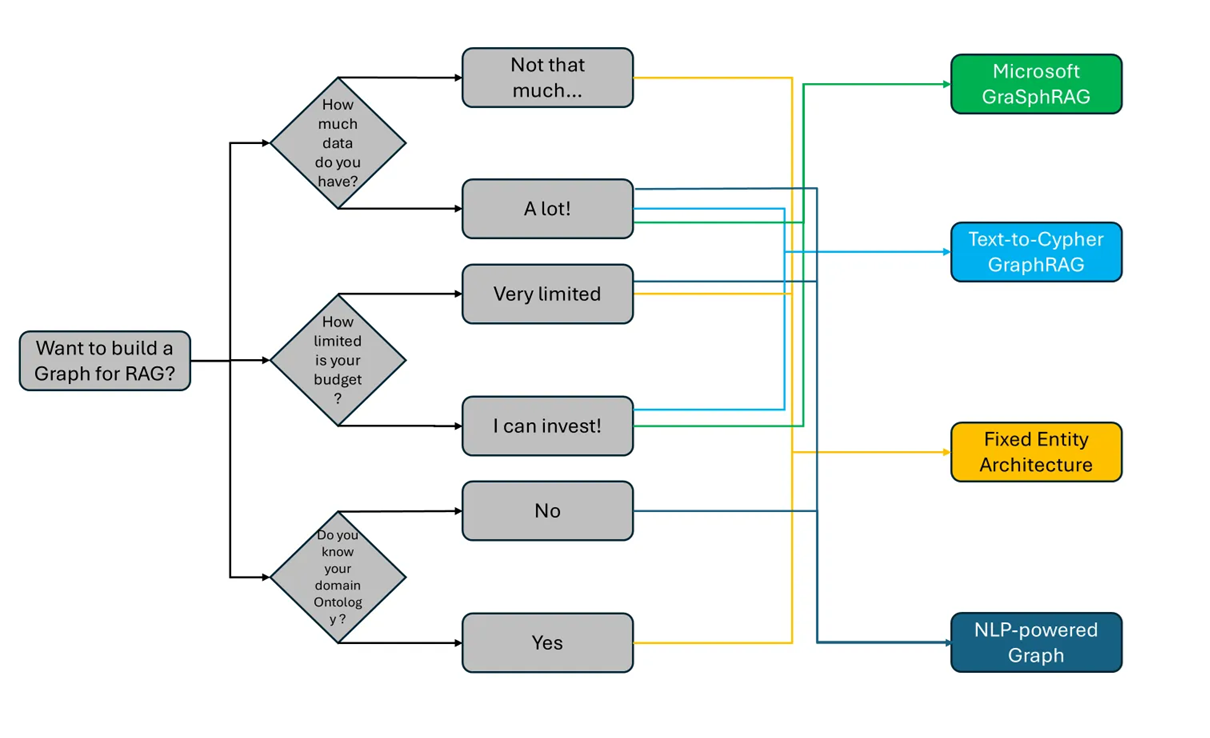
\includegraphics[width=\linewidth,keepaspectratio]{graphrag1}
	
	% {\tiny (Ref: Build your hybrid-Graph for RAG \& GraphRAG applications using the power of NL - Irina Adamchic)}
	% \end{center}
	
% \end{frame}


% %%%%%%%%%%%%%%%%%%%%%%%%%%%%%%%%%%%%%%%%%%%%%%%%%%%%%%%%%%%
% \begin{frame}[fragile]\frametitle{Neo4j Ollama GraphRAG}

	% \begin{center}
	% 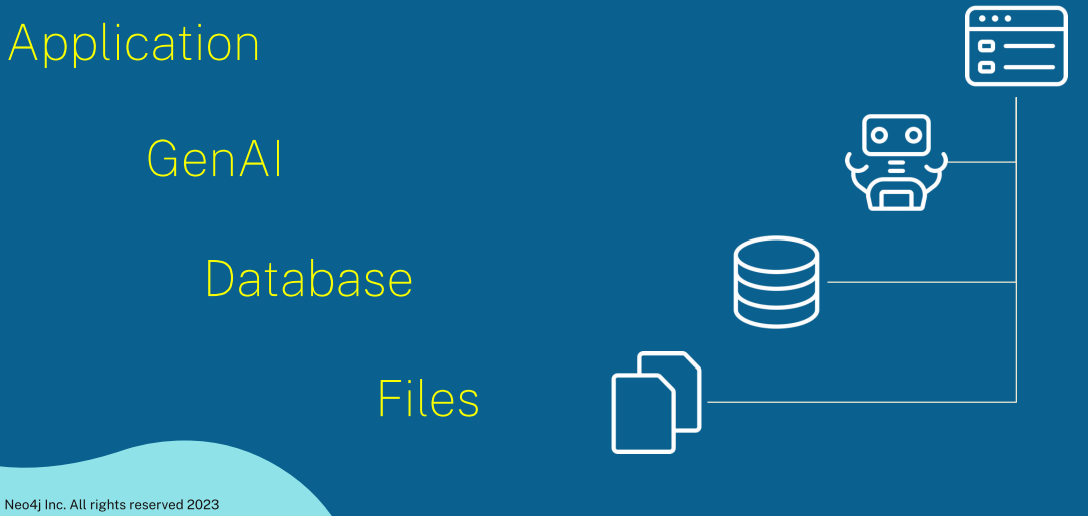
\includegraphics[width=0.6\linewidth,keepaspectratio]{graphrag2}
	
	% {\tiny (Ref: The GenAI Stack - Andreas Kollegger - Neo4j)}
	% \end{center}
	
	    % \begin{itemize}
        % \item Application: LangChain: an ``orchestration framework'' for integrating with LLMs
		% \item Gen AI : Ollama : locally managed language models
		% \item Database: Neo4j: knowledge graph to augment the LLM
		% \item Files: import: sample data sources for constructing a knowledge graph
    % \end{itemize}
% \end{frame}

%%%%%%%%%%%%%%%%%%%%%%%%%%%%%%%%%%%%%%%%%%%%%%%%%%%%%%%%%%%%%%%%%%%%%%%%%%%%%%%%%%
\begin{frame}[fragile]\frametitle{}
\begin{center}
{\Large Code Walkthrough: Medical Doc Analysis with Fast GraphRAG}

	{\tiny (Ref: GraphRAG: The Practical Guide for Cost-Effective Document Analysis with Knowledge Graphs -Jaykumaran)}
	
\end{center}
\end{frame}


%%%%%%%%%%%%%%%%%%%%%%%%%%%%%%%%%%%%%%%%%%%%%%%%%%%%%%%%%%%
\begin{frame}[fragile]\frametitle{FastGraphRAG Overview}
    \begin{itemize}
        \item All functions are asynchronous, enabling concurrent API calls.
        \item Works well with providers without RPM limits (e.g., OpenAI).
    \end{itemize}
\end{frame}

%%%%%%%%%%%%%%%%%%%%%%%%%%%%%%%%%%%%%%%%%%%%%%%%%%%%%%%%%%%
\begin{frame}[fragile]\frametitle{Installation}
    \begin{lstlisting}
    !git clone https://github.com/circlemind-ai/fast-graphrag.git
    %cd fast_graphrag
    %poetry install
    
    # or
    !pip install fast-graphrag
    \end{lstlisting}
\end{frame}

%%%%%%%%%%%%%%%%%%%%%%%%%%%%%%%%%%%%%%%%%%%%%%%%%%%%%%%%%%%
\begin{frame}[fragile]\frametitle{Importing Dependencies}
    \begin{lstlisting}
    import instructor  # Structured outputs for LLMs
    import os
    from fast_graphrag import GraphRAG, QueryParam
    from fast_graphrag._llm import OpenAIEmbeddingService, OpenAILLMService
    \end{lstlisting}
\end{frame}

%%%%%%%%%%%%%%%%%%%%%%%%%%%%%%%%%%%%%%%%%%%%%%%%%%%%%%%%%%%
\begin{frame}[fragile]\frametitle{Dataset: MIMIC-IV-ICU}
    \begin{itemize}
        \item Public dataset of de-identified ICU patient EHRs.
        \item Using first 430 samples (~650 words per file).
    \end{itemize}
    \begin{lstlisting}
    mimic_ex_500/
    |- report_0.txt
    |- report_1.txt
    |-  ... 
    |- report_499.txt
    |- report_500.txt
    \end{lstlisting}
\end{frame}

%%%%%%%%%%%%%%%%%%%%%%%%%%%%%%%%%%%%%%%%%%%%%%%%%%%%%%%%%%%
\begin{frame}[fragile]\frametitle{Defining Domain and Entity Types}
    \begin{lstlisting}[language=markdown]
    DOMAIN = "Analyze clinical records for key medical entities."
	EXAMPLE_QUERIES = [
		"What are the common risk factors for sepsis in ICU patients?",
		"How do trends in lab results correlate with patient outcomes in cases of acute kidney injury?",
		"Describe the sequence of interventions for patients undergoing major cardiac surgery.",
		"How do patient demographics and comorbidities influence treatment decisions in the ICU?",
		"What patterns of medication usage are observed among patients with chronic obstructive pulmonary disease (COPD)?"]	
    ENTITY_TYPES = ["Patient", "Diagnosis", "Procedure", "Lab Test", "Medication", "Outcome", "Unknown"]
    working_dir = "./WORKING_DIR/mimic_ex500/"
    \end{lstlisting}
\end{frame}

%%%%%%%%%%%%%%%%%%%%%%%%%%%%%%%%%%%%%%%%%%%%%%%%%%%%%%%%%%%
\begin{frame}[fragile]\frametitle{Configuring the FastGraphRAG Pipeline}
    \begin{lstlisting}
grag = GraphRAG(
    working_dir=working_dir,
    n_checkpoints=2, # to save backups (recommended)
    domain=DOMAIN,
    example_queries="\n".join(EXAMPLE_QUERIES),
    entity_types=ENTITY_TYPES,
    config=GraphRAG.Config(
        llm_service=OpenAILLMService(
            model="Phi4_6k",  # gemini-2.0-flash-exp
            # or https://generativelanguage.googleapis.com/v1beta/openai/
            base_url="http://localhost:11434/v1",  # Ollama
            api_key="ollama",  # or GEMINI_API_KEY
            mode=instructor.Mode.JSON,
            client="openai"),
        embedding_service=OpenAIEmbeddingService(
            model="mxbai-embed-large",  # mxbai-embed-large
            base_url="http://localhost:11434/v1",
            api_key="ollama",
            embedding_dim=1024,  # mxbai-embed-large - 1024 ; nomic-embed - 768
            client="openai"),
    ),
)
directory_path = "mimic_ex_430" # input dir to the dataset
    \end{lstlisting}
\end{frame}


%%%%%%%%%%%%%%%%%%%%%%%%%%%%%%%%%%%%%%%%%%%%%%%%%%%%%%%%%%%
\begin{frame}[fragile]\frametitle{Graph Indexing}
    \begin{lstlisting}
def graph_index(directory_path):
    file_count = 0 # Keep track of processed files.
    for filename in os.listdir(directory_path):
        if filename.endswith('.txt'):
            file_path = os.path.join(directory_path, filename)
            with open(file_path, 'r') as file:
                content = file.read()
                if isinstance(content, list):
                    content = "\n".join(map(str, content))
                if isinstance(content, dict):
                    key_to_use = next(iter(content.keys()), None)
                    content = content[key_to_use] if key_to_use else str(content)
                else: content = str(content)   
                grag.insert(content)
            file_count += 1
            total_files = sum(1 for f in os.listdir(directory_path) if f.endswith(".txt"))
            print("******************** $$$$$$ *****************")        
            print(f"Total Files Processed: -> {file_count} / {total_files}")
            print("******************** $$$$$$ *****************")  
    return None
graph_index(directory_path)
    \end{lstlisting}
\end{frame}

%%%%%%%%%%%%%%%%%%%%%%%%%%%%%%%%%%%%%%%%%%%%%%%%%%%%%%%%%%%
\begin{frame}[fragile]\frametitle{Indexing Performance}
    \begin{itemize}
        \item Indexed 430 items in ~510 minutes (8.5 hours).
        \item Processed locally with a 14B model.
    \end{itemize}
\end{frame}

%%%%%%%%%%%%%%%%%%%%%%%%%%%%%%%%%%%%%%%%%%%%%%%%%%%%%%%%%%%
\begin{frame}[fragile]\frametitle{Querying Example 1: Targeted at Global}
    \begin{lstlisting}[language=markdown]
    grag.query("Describe the sequence of interventions for cardiac surgery?").response

**********************************************
The sequence of interventions for the clinical scenario in post-aortic valve repair surgery with complications like respiratory issues, neurological impairment, and renal failure includes:
**Pre-surgery Preparation:**
- Evaluate and stabilize the patient.
**Intraoperative Procedures:**
- Conduct aortic valve replacement or repair.
**Immediate Postoperative Care:**
- Continue invasive mechanical ventilation, especially in patients with respiratory issues or neurological impairments preoperatively.
    \end{lstlisting}

\end{frame}

%%%%%%%%%%%%%%%%%%%%%%%%%%%%%%%%%%%%%%%%%%%%%%%%%%%%%%%%%%%
\begin{frame}[fragile]\frametitle{Querying Example 1: Targeted at Global}
    \begin{lstlisting}[language=markdown]
**Rehabilitation and Follow-up:**
- Perform swallow evaluation tests to ensure readiness for oral intake, followed by a diet progression to soft or clear liquids if necessary.
 
**Commonly Used Medications:**
- Anticoagulants (e.g., heparin) to prevent blood clots.

 A multidisciplinary team including cardiologists, pulmonologists, and other specialists is often involved to address any comorbid conditions.
**********************************************
 
# o3-mini-high rated this response : 8/10.	
    \end{lstlisting}

\end{frame}

%%%%%%%%%%%%%%%%%%%%%%%%%%%%%%%%%%%%%%%%%%%%%%%%%%%%%%%%%%%
\begin{frame}[fragile]\frametitle{Querying Example 2: Targeted at Global}
    \begin{lstlisting}[language=markdown]
    grag.query("How do demographics and comorbidities influence ICU decisions?").response
	
**********************************************
Patient demographics and comorbidities significantly influence treatment decisions in the ICU, as evidenced by detailed hospital courses described in various scenarios.
 
1. **Demographics**: Specific ages or life stages, such as "on day of life 45" for a patient with unique medical conditions (metabolic issues), indicate tailored care plans sensitive to developmental stages.
 
2. **Comorbidities**:
   - A history like short gut syndrome and colectomy influences decisions about when and how to restart total parenteral nutrition (TPN). \ldots .	
    \end{lstlisting}

\end{frame}

%%%%%%%%%%%%%%%%%%%%%%%%%%%%%%%%%%%%%%%%%%%%%%%%%%%%%%%%%%%
\begin{frame}[fragile]\frametitle{Querying Example 2: Targeted at Global}
    \begin{lstlisting}[language=markdown]
3. **Interactions**: Decisions like replacing a PICC line with a Hickman catheter after infection shows proactive steps in avoiding repeat complications due to prior infections from central lines.
4. **Treatment Customization**: The management decisions, such as adjusting insulin administration for endocrine challenges even when insulin levels are normal, demonstrate personalized ICU therapy adapting for nuanced metabolic control in conditions like hypoglycemia of unknown origin.
    
These scenarios highlight that ICU treatment is deeply influenced by a patient's demographic specifics \ldots and chronic health issues effectively.
**********************************************
# o3-mini-high rated this response : 8/10.	
    \end{lstlisting}

\end{frame}


%%%%%%%%%%%%%%%%%%%%%%%%%%%%%%%%%%%%%%%%%%%%%%%%%%%%%%%%%%%
\begin{frame}[fragile]\frametitle{Querying Example 3: Targeted at Global}
        \begin{lstlisting}[language=markdown]
    grag.query("How can lung function be improved in COPD + Heart Failure?").response
	
**********************************************
To optimize the treatment for patients with both COPD and heart failure, it is crucial to manage fluids carefully using diuretics without causing respiratory issues. This necessitates precise adjustments in medication dosages, closely monitoring fluid balance, and ensuring proper oxygenation levels. Right heart catheterization can assist in measuring cardiac function and tailoring treatments for these patients. The goal is to alleviate symptoms of both conditions while preventing exacerbations, which often involves using supplemental oxygen or bronchodilators as required.
**********************************************
# o3-mini-high rated this response : 8/10.	
    \end{lstlisting}

\end{frame}

%%%%%%%%%%%%%%%%%%%%%%%%%%%%%%%%%%%%%%%%%%%%%%%%%%%%%%%%%%%
\begin{frame}[fragile]\frametitle{Querying Example 4: Targeted at Local}
        \begin{lstlisting}[language=markdown]
    grag.query("Discuss Hypocapnic and Hypoxemic Respiratory Failure").response
	
Hypocapnic Respiratory Failure and Hypoxemic Respiratory Failure are two distinct categories of respiratory failure, each characterized by different clinical features. Conversely,\ldots Accurate assessment and differentiation between these conditions are crucial for appropriate management and treatment.

In medical practice, both types may coexist or require different clinical interventions based on the specific underlying pathology.
**********************************************
# o3-mini-high rated this response : 6/10.	
    \end{lstlisting}

\end{frame}


%%%%%%%%%%%%%%%%%%%%%%%%%%%%%%%%%%%%%%%%%%%%%%%%%%%%%%%%%%%
\begin{frame}[fragile]\frametitle{FastGraphRAG Performance}
    \begin{itemize}
        \item 27x faster and 40\% more accurate retrieval.
        \item Benchmarks (2wikimultihopQA, 101 queries):
    \end{itemize}

	
    \begin{tabular}{lccc}
        \hline
        Method & Accuracy (All) & Accuracy (Multihop) & Insertion Time (min) \\
        \hline
        VectorDB & 0.42 & 0.23 & $\sim$0.3 \\
        LightRAG & 0.45 & 0.28 & $\sim$25 \\
        GraphRAG & 0.73 & 0.64 & $\sim$40 \\
        FastGraphRAG & 0.93 & 0.90 & $\sim$1.5 \\
        \hline
    \end{tabular}	
	
	{\tiny (Ref: GraphRAG: The Practical Guide for Cost-Effective Document Analysis with Knowledge Graphs -Jaykumaran)}	
\end{frame}


%%%%%%%%%%%%%%%%%%%%%%%%%%%%%%%%%%%%%%%%%%%%%%%%%%%%%%%%%%%
\begin{frame}[fragile]\frametitle{FastGraphRAG at Inference Time}
    \begin{itemize}
        \item Uses a PageRank-like algorithm (similar to Google).
        \item Determines importance of elements in the KG.
        \item Retrieves only the most relevant entities and relationships.
        \item Produces high-quality, precise responses.
    \end{itemize}
\end{frame}

%%%%%%%%%%%%%%%%%%%%%%%%%%%%%%%%%%%%%%%%%%%%%%%%%%%%%%%%%%%
\begin{frame}[fragile]\frametitle{Evaluating FastGraphRAG for Your Use Case}
    \begin{itemize}
        \item Consider cost-to-performance ratio for your specific dataset.
        \item Assess viability based on document complexity and enterprise needs.
        \item FastGraphRAG offers a scalable approach with efficiency gains.
    \end{itemize}
\end{frame}

%%%%%%%%%%%%%%%%%%%%%%%%%%%%%%%%%%%%%%%%%%%%%%%%%%%%%%%%%%%
\begin{frame}[fragile]\frametitle{Limitations of FastGraphRAG}
    \begin{itemize}
        \item Asynchronous and Pydantic-validated, challenging for beginners.
        \item 7B-class models struggle with structured responses.
        \item Limited documentation and community support.
        \item LightRAG offers better support for local LLMs.
        \item Faster than GraphRAG/LightRAG but slower than vector-only RAG.
        \item Best for large datasets and high-stakes domains.
        \item For simple use cases, vector-only RAG is recommended.
    \end{itemize}
\end{frame}

%%%%%%%%%%%%%%%%%%%%%%%%%%%%%%%%%%%%%%%%%%%%%%%%%%%%%%%%%%%
\begin{frame}[fragile]\frametitle{Trivia: PDF Indexing Challenges}
    \begin{itemize}
        \item Faced issues with PDF indexing using pdf-plumber.
        \item Pydantic validation errors encountered.
        \item Works fine with .txt files converted from PDFs.
        \item Did not extensively debug the issue.
    \end{itemize}
\end{frame}

%%%%%%%%%%%%%%%%%%%%%%%%%%%%%%%%%%%%%%%%%%%%%%%%%%%%%%%%%%%
\begin{frame}[fragile]\frametitle{Conclusion}
    \begin{itemize}
        \item GraphRAG enables tracking patient behavioral patterns.
        \item Supports complex, multi-hop queries with accurate responses.
        \item Ideal for high-stakes domains requiring precision.
        \item Knowledge graphs improve reasoning and interpretability.
        \item Hybrid approaches (KG + vectors) outperform naive RAG.
    \end{itemize}
\end{frame}





